\documentclass[12pt]{article}

\usepackage[english]{babel}

% Math/Greek packages
\usepackage{amssymb,amsmath,amsthm, mathtools} 
\usepackage{algorithm, algorithmic}
\usepackage{upgreek, siunitx}

% Graphics/Presentation packages
\usepackage{geometry, graphicx}
\usepackage{tabulary, enumitem, array}
\usepackage{xparse,mleftright,tikz}
\usepackage{physics}

% Misc packages
\usepackage{fancyhdr}


\usepackage[export]{adjustbox}

\usepackage{esint}

\sisetup{locale=US,group-separator = {,}}
\usepackage[colorlinks=true, allcolors=blue]{hyperref}


% Box function - update this as more sophisticated solutions are found
\newcommand\mybox[2][]{\tikz[overlay]\node[fill=blue!20,inner sep=2pt, anchor=text, rectangle, rounded corners=1mm,#1] {#2};\phantom{#2}}
\renewcommand{\arraystretch}{1.2}

% General macro declarations


\makeatletter
\let\oldabs\abs
\def\abs{\@ifstar{\oldabs}{\oldabs*}}
%
\let\oldnorm\norm
\def\norm{\@ifstar{\oldnorm}{\oldnorm*}}
\makeatother

\begin{document}

\title{PHSX 461: HW11}
\author{William Jardee}
\maketitle

\section*{Griffiths 4.12}
{\sl Work out the radial wave functions of $R_{31}$, using the recursion formula. Don't bother to normalize them.}

\begin{equation}
	\tag{Equation 4.76}
	c_{j+1} = \frac{2(j+l+1-n)}{(j+1)(j+2l+2)}c_j
	\label{eq:4.76}
\end{equation}

\[R_{n, l} = \frac{1}{r}\rho^{l+1}e^{-r/a}V_n\Big(\frac{r}{a}\Big)\]
\[\Rightarrow R_{3,1} = \frac{1}{r}\Big(\frac{r}{3a}\Big)^2 \Big[c_0 + c_1 \Big(\frac{r}{3a}\Big) + c_2 \Big(\frac{r}{3a}\Big)^2\Big]\]
taking a quick break to calculate c's:
\[c_0 = c_0\]
\[c_1 = \frac{2(0+1+1-3)}{(0+1)(0+2+2)}c_0 = -\frac{1}{2}c_0\]
\[c_2 = \frac{2(1+1+1-3)}{(1+1)(1+2+2)}c_1 = 0\]
Plugging these back in:
\[\boxed{R_{3,1} = \frac{c_0 r}{(3a)^2}\Big[1 - \frac{1}{2} \Big(\frac{r}{3a}\Big)\Big]}\]

\newpage
%-------------------------------------------------------------

\section*{Griffiths 4.15}
\begin{enumerate}[label=\alph*)]
\item {\sl Find $\ev{r}$ and $\ev{r^2}$ for an electron in the ground state of hydrogen. Express your answers in terms of the Bohr radius.}

\[\ev{r} \Rightarrow \ev{r}{\psi} = \ev{r}{R_{10}} = \int(4a^{-3}r\exp(-2r/a))r^2\dd{r}\]
\[\boxed{\ev{r} = 0} \quad \text{(odd)}\]

\[\ev{r^2} \Rightarrow \ev{r^2}{\psi} = \ev{r^2}{R_{10}} = \int_{-\infty}^\infty 4a^{-3}r^2 \exp(-er/a)r^2\dd{r} \]
\[ = 8a^{-3}\int_0^\infty r^4 \exp(-er/a) \dd{r} \quad \text{(even)}\]
By using an identity given in Griffiths
\[= 8a^{-3}\Big(4!\Big(\frac{a}{2}\Big)^5\Big)\]
\[\boxed{\ev{r^2} = 24 a^2}\]

\item {\sl Find $\ev{x}$ and $\ev{x^2}$ for an electron in the ground state of hydrogen.}

There is no bias in the location for $n=1$, so the expected $r$ will be a symmetric sphere. Thus, $\boxed{\ev{x} = 0}$

We know that $\ev{r^2} = \ev{x^2 + y^2 + z^2} = \ev{x^2} + \ev{y^2} + \ev{z^2}$. Since the spherical harmonic is symmetric in $\theta$ and $\phi$ for the $n=1$ level, then all three components will be equal. Thus:
\[\ev{r^2} = 3\ev{x^2} \rightarrow \boxed{\ev{x^2} = 8a^2}\]

\item {\sl Find $\ev{x^2}$ in the state $n=2, l=1, m=1$.}
The quickest way for me to do with, was to just do it. 
\[\ev{x^2} = \ev{x^2}{\psi} = \ev{(r\sin(\theta)\cos(\phi))^2}{\psi}\]
since we are at $n=2,l=1,m=1$, we can just read $\psi$ out of the book. 
\[R_{2,1}Y^1_1 = \Big[\frac{1}{2\sqrt{6}}a^{-3/2}\Big(\frac{r}{a}\Big)\exp(-2r/a)\Big]
\Big[-\Big(\frac{3}{4\pi}\Big)^{1/2}\cos\theta \Big]\]\smallskip
\[\ev{x^2} = \int r^2 \frac{1}{2\sqrt{6}}a^{-3}\Big(\frac{r}{a}\Big)\exp(-r/a) r^2 \dd{r} \cdot\]
\[\int -\Big(\frac{3}{4\pi}\Big)\cos^2\theta \sin^2 \theta \cos^2\phi \sin\theta \dd{\theta} \dd{\phi}\]
\[= \Big(\frac{3}{4 \pi}\Big)\frac{1}{24}a^{-3}\Big(\frac{1}{a^2}\Big)\int r^6 \exp(-r/a)\dd{r} \int \cos^2 \theta \sin^3 \theta cos^2 \phi \dd{\theta} \dd{\phi}\]
\[= \frac{1}{32 \pi}\Big(\frac{1}{a^5}\Big)(6!(a)^7) \int^{\pi}_0 (\cos^2 \theta - \cos^4 \theta)\sin \theta \dd{\theta} \int^{2 \pi}_0 \frac{1}{2}(1 + \cos 2\phi) \dd{\phi}\]
\[= \frac{6!}{32 \pi}a^2 \Big[\frac{1}{3}\cos^3 \theta - \frac{1}{5} \cos^5 \theta\Big]\eval_0^\pi \Big[\frac{1}{2}\phi + \frac{1}{4}\sin 2\phi\Big]\eval_0^{2\pi}\]
\[= \frac{6!}{32 \pi}a^2 \Big[\frac{4}{16}\Big]\pi\]
\[= \frac{45}{8}a^2\]
\[\boxed{\ev{x^2} = \frac{45}{8}x^2}\]

\end{enumerate}

\newpage
%-------------------------------------------------------------

\section*{Griffiths 4.16}
{\sl What is the most probably value of r, in the ground state of hydrogen?}

\[\psi \propto R_{1,0} = 2a^{-3/2}\exp(-r/a)\]
\[P = \psi^* \psi \propto 4a^{-3} \exp(-r/a)r^2\]
\[P(r) = \psi^* r \psi \propto \frac{4}{a^3}r^3 \exp(-r/a)\]
\begin{figure}[!ht]
\centering
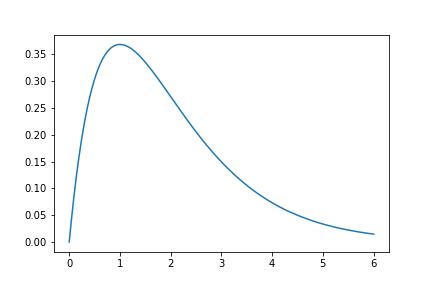
\includegraphics[scale=.75]{hw11_3.png}
\caption{The graph for Question 4.16}
\end{figure}
So, we need to take the derivative to find where that max is:
\[3r^2 \frac{4}{a^3}\exp(-r/a) - \frac{4}{a^3}\frac{r^3}{a} \exp(-r/a) = 0\]
\[\frac{12}{a^3} - \frac{4}{a^4}r = 0\]
\[3 -\frac{1}{a}r = 0\]
\[\boxed{r = 3a}\]

\newpage
%-------------------------------------------------------------

\section*{Griffiths 4.27}
{\sl Two particles $($masses $m_1$ and $m_2)$ are attached to the ends of a massless rigid rod of length $a$. the system is free to rotate in three dimensions about the $($fixed$)$ center of mass.}
\begin{enumerate}[label=\alph*)]
\item {\sl Show that the allowed energies of this rigid rotor are}

\[E_n = \frac{\hbar^2}{2I}n(n+1) \quad (n = 0,1,2,...) \quad \text{where } I = \frac{m_1 m_2}{m_1 + m_2}a^2\]
{\sl is the moment of inertia of the system}

Normally $T = \frac{L^2}{2I}$, so the operator is then $\hat{T} = \frac{1}{2I}(\hat{L})^2$. 
\[\hat{T}\ket{\psi} = \frac{1}{2I}\hat{L}^2 \ket{\psi} = \frac{1}{2I}\hbar^2 n(n+1) \ket{\psi}\]
Since, we don't have any potential function, then the eigenvalue of the energy is $\boxed{E_n = \frac{\hbar^2}{2I}n(n+1)}$

\item {\sl What are the normalized eigenfunctions for this system? $($Let $\theta$ and $\phi$ define the orientation of the rotor axis.$)$ What is the degeneracy of the $n$th energy level?}

These have the same eigenvalues of $\hat{L}^2$, so the eigenfunctions will be the spherical harmonics: $\boxed{Y_1^1(\theta, \phi)}$. If we think of the spherical harmonics, there is kinda a hidden $m$ value here, that can go from $-n, -n+1, ... n-1, n$. There are 2n+1 values here. So, it is this is $\boxed{2n+1 \text{ degenerate}}$

\item {\sl What spectrum would you expect for this system?}

Let's take two consecutive energies, $n$ and $n+1$
\[\nu = \frac{E_{n+1}-E_n}{2\pi} = \frac{1}{2 \pi}\Big(\frac{\hbar}{2I}(n+1)(n+2) - \frac{\hbar}{2I}n(n+1)\Big) = \frac{\hbar}{2 \pi I}(n+1)(n+2-n)\]
\[\boxed{\nu = \frac{\hbar}{2 \pi I}j \text{ where } j = n+1}\]

\item {\sl According to the figure given in the text, what is the frequency separation between adjacent lines? Look up the masses of $^{12}C$ and $^{16}O$, and from $m_1$, $m_2$, and $\Delta \nu$ determine the distance between the atoms.}

There are 5 lines between 30 and 50, so $\Delta\nu \approx 4 \text{cm}^{-1}$. By ``googling", 
$^{12}C \rightarrow m_1 \approx 1.9927e^{-23}$g and $^{16}O \rightarrow m_2 = 2.6593e^{-23}$g.
Solving for $a$:
\[a = \sqrt{\frac{8\pi}{\hbar}\Big(\frac{1}{m_1} + \frac{1}{m_2}\Big)}\]
\[\boxed{a \approx 1.9193 \mu \text{m}}\]

\end{enumerate}

\newpage
%-------------------------------------------------------------

\section*{Griffiths 4.64}
{\sl the electron in a hydrogen atom occupies the combined spin and position state}

\[R_{21}(\sqrt{1/3}Y^0_1 \chi_+ + \sqrt{2/3}Y^1_1 \chi_-)\]
\begin{enumerate}[label=\alph*)]
\item {\sl If you measured the orbital angular momentum squared, what values might you get, and what is the probability of each? }

The magnitude of angular momentum is only dependent on $l$, 
\[L^2 \ket{l,m} = l(l+1)\hbar^2 \ket{l,m}\]
So there is only one value possible, with value $\boxed{2\hbar^2}$

\item {\sl Same for the $z$ component of angular momentum.}

Same kinda thing as above:
\[L_z \ket{l,m} = m\hbar \ket{l,m}\]
\[\boxed{0 \text{ with probability } \frac{1}{3}, \hbar \text{ with probability } \frac{2}{3}}\]

\item {\sl Same for the spin angular momentum squared.}

\[S^2\ket{s, m_s} = s(s+1)\hbar^2 \ket{s, m_s}\]
\[\boxed{\text{One possible value } \frac{3}{4}\hbar^2}\]

\item {\sl Same for the $z$ component of spin angular momentum.}

\[S_z \ket{s, m_s} = m_s \hbar \ket{s, m_s}\]
\[\boxed{\frac{\hbar}{2} \text{ with probability } \frac{1}{3}, -\frac{\hbar}{2} \text{ with probability } \frac{2}{3}}\]

\item {\sl Same for the energy of the electron.}

\[\hat{H}\ket{n} = -\Big[\frac{m_e}{2\hbar}\Big(\frac{e^2}{4\pi \varepsilon_0}\Big)\Big]\frac{1}{n^2}\ket{n}\]
\[\text{Since } n=1\rightarrow \boxed{E_1 = -\frac{m_e}{2\hbar}\frac{1}{4}\Big(\frac{e^2}{4\pi\varepsilon_0}\Big)^2}\]

\end{enumerate}

\newpage
%-------------------------------------------------------------

\section*{Griffiths 4.30}
{\sl An electron is in the spin state}
\[\chi = A \mqty(3i & 4)\]
\begin{enumerate}[label=\alph*)]
\item {\sl Determine the normalization constant $A$}
\[(9+16)A^2 = 1 \rightarrow \boxed{A = \frac{1}{5}}\]

\item {\sl Find the expectation values of $S_x$, $S_y$, and $S_z$}

Since our spin state is given in the $z$ basis, we can just read those off: 
\[\frac{9}{25}\frac{\hbar}{2} - \frac{16}{25}\frac{\hbar}{2} = -\frac{7}{25}\frac{\hbar}{2}\]
\[\boxed{\ev{S_z} = -\frac{7}{25}\frac{\hbar}{2}}\]

\[\ev{S_y} = \chi^\dagger S_y \chi = \frac{1}{5}\mqty(-3i & 4)\frac{\hbar}{2}\mqty(0 & -i \\ i & 0)\frac{1}{5}\mqty(3i \\ 4)\]
\[\boxed{\ev{S_y} = -\frac{24}{25}\frac{\hbar}{2}}\]

\[\ev{S_x} = \chi^\dagger S_x \chi = \frac{1}{5}\mqty(-3i & 4)\frac{\hbar}{2}\mqty(0 & 1 \\ 1 & 0)\frac{1}{5}\mqty(3i \\ 4)\]
\[\boxed{\ev{S_x} = 0}\]

\item {\sl Find the ``uncertainties" $\sigma_{S_x}$, $\sigma_{S_y}$, and $\sigma_{S_z}$}

We know that $\sigma_x^2 = \ev{x^2} - \ev{x}^2$. Sp, now we just need to know $\hat{S_z}^2$, etc. 
\[S_z^2 = S_z S_z = \Big(\frac{\hbar}{2}\Big)^2\mqty(1 & 0 \\ 0 & -1) \mqty(1 & 0 \\ 0 & -1) = \Big(\frac{\hbar}{2}\Big)^2\mqty(1 & 0 \\ 0 & 1)\]
\[S_y^2 = S_y S_y = \Big(\frac{\hbar}{2}\Big)^2\mqty(0 & -i \\ i & 0) \mqty(0 & -i \\ i & 0) = \Big(\frac{\hbar}{2}\Big)^2\mqty(1 & 0 \\ 0 & 1)\]
\[S_x^2 = S_x S_x = \Big(\frac{\hbar}{2}\Big)^2\mqty(0 & 1 \\ 1 & 0) \mqty(0 & 1 \\ 1 & 0) = \Big(\frac{\hbar}{2}\Big)^2\mqty(1 & 0 \\ 0 & 1)\]

Since $S_x^2 = S_y^2 = S_z^2 \Longrightarrow \ev{S_x^2} = \ev{S_y^2} = \ev{S_z^2}$.

\[\ev{\chi}{S_z} \Rightarrow \frac{1}{5}\mqty(-3i & 4)\Big(\frac{\hbar}{2}\Big)^2\mqty(1 & 0 \\ 0 & -1)\frac{1}{5}\mqty(3i \\ 4) = \Big(\frac{\hbar}{2}\Big)^2\]
\[\boxed{\sigma_{S_z} = \sqrt{\ev{S_z^2}- \ev{S_z}^2} = \frac{\hbar}{2}\sqrt{1-\Big(-\frac{7}{25}\Big)^2}}\]\smallskip

\[\boxed{\sigma_{S_y} = \sqrt{\ev{S_y^2}- \ev{S_y}^2} = \frac{\hbar}{2}\sqrt{1-\Big(-\frac{24}{25}\Big)^2}}\]\smallskip

\[\boxed{\sigma_{S_x} = \sqrt{\ev{S_x^2}- \ev{S_x}^2} = \frac{\hbar}{2}\sqrt{1-0} = \frac{\hbar}{2}}\]\smallskip

\item {\sl Confirm that your results are consistent with all three uncertainty principles.}
The one they are referring to is
\[\sigma_{L_x}\sigma_{L_y} \geq \frac{\hbar}{2}\abs{\ev{L_z}}\]

\[\sigma_{S_x}\sigma_{S_x} = \Big(\frac{\hbar}{2}\Big)^2\sqrt{1- \Big(\frac{24}{25}\Big)^2} = 0.28 \Big(\frac{\hbar}{2}\Big)^2 \geq \frac{\hbar}{2}\Big|-\frac{7}{25}\frac{\hbar}{2}\Big| = 0.28 \Big(\frac{\hbar}{2}\Big)^2 \quad \checkmark\]

\[\sigma_{S_y}\sigma_{S_z} = \Big(\frac{\hbar}{2}\Big)^2\sqrt{1- \Big(\frac{24}{25}\Big)^2}\sqrt{1- \Big(\frac{7}{25}\Big)^2} = 0.269 \Big(\frac{\hbar}{2}\Big)^2 \geq \frac{\hbar}{2}|0| = 0 \quad \checkmark\]

\[\sigma_{S_z}\sigma_{S_x} = \Big(\frac{\hbar}{2}\Big)^2\sqrt{1- \Big(\frac{7}{25}\Big)^2} = 0.96 \Big(\frac{\hbar}{2}\Big)^2 \geq \frac{\hbar}{2}\Big|-\frac{24}{25}\frac{\hbar}{2}\Big| = 0.96 \Big(\frac{\hbar}{2}\Big)^2 \quad \checkmark\]

\end{enumerate}

\end{document}